\chapter{Estado de la Cuestión}
\label{cap:estadoDeLaCuestion}



\begin{resumen} En este capítulo se dará una idea general sobre los Sistemas aumentativos y alternativos de comunicación \ref{cap3:sec:saac}, las características de los pictogramas y los distintos sistemas pictográficos que existen \ref{cap3:sec:pictogramas}. Finalmente, se verán las distintos herramientas con las que se construyen tableros de pictogramas \ref{cap3:sec:editor-tableros}.

\end{resumen}


Los humanos siempre  han tenido la necesidad inherente de comunicarse y quien no es capaz de hacerlo generalmente acaba excluido. A día de hoy este problema sigue afectando a parte de la población como es el caso de las personas con Trastorno del Espectro Autista (\textit{TEA}).
\\

Sin entrar en gran detalle, podemos encontrar que la gente con \textit{TEA} tiene dificultades en la comunicación verbal, pues a menudo ésta no es recíproca o no se realiza en el contexto social adecuado. Respecto a la comunicación no verbal, también sufren dificultades al entender el significado de gestos faciales o expresión corporal de otras personas. Todo esto causa a menudo malentendidos, pues generalmente no se comprende el contexto y dificulta la comunicación. 


\section{Sistemas Aumentativos y Alternativos de Comunicación}
\label{cap3:sec:saac}
Los Sistemas Aumentativos y Alternativos de Comunicación (\textit{SAAC}) son las distintas formas de expresión sin tener en cuenta el lenguaje hablado que tiene como finalidad aumentar y/o compensar los problemas de comunicación de personas con discapacidad como por ejemplo trastornos del espectro autista, discapacidad intelectual, deficiencia auditiva, parálisis cerebral entre otros.

En ocasiones puede hacer falta el uso de recursos para poder comunicarse, es por ello que podemos distinguir dos tipos de \textit{SAAC}, los sistemas sin ayuda y los sistemas con ayuda.
\newpage
\begin{itemize}
	\item \textbf{Sistemas sin ayuda}: no utilizan ningún recurso externo para establecer la comunicación, únicamente usan su propio cuerpo. En los sistemas sin ayuda podemos observar dos tipos de grupos, los métodos gestuales (lengua de signos) y los métodos oralistas (lectura labiofacial). 
	\item \textbf{Sistemas con ayuda}: utilizan recursos externos para establecer la comunicación. Los más utilizados suelen ser pictogramas, imágenes o símbolos.
\end{itemize}

Las \textit{SAAC} utilizan múltiples recursos para poder comunicarse con personas con discapacidades cognitivas y entre todos ellos destacan los sistemas pictográficos. Se trata de uno de los sistemas más utilizados y esto es debido a su fácil comprensión ya que representan gráficamente lo que se desea transmitir como palabras o conceptos. 

\section{Pictogramas}
\label{cap3:sec:pictogramas}
Los pictogramas son imágenes o símbolos de rápida comprensión que expresan acciones, objetos, emociones, etc. Un conjunto de pictogramas en un cierto orden, pueden generar una oración. Todos ellos deben cumplir las siguientes características:
\begin{enumerate}
	\item \textbf{Referencialidad}: relación del pictograma con el referente.
	\item \textbf{Ítems gráficos}: imágenes que representen de manera sencilla aquello que se toma como modelo.
	\item \textbf{Comprensión}: debe ser fácilmente entendible independientemente de la formación, idioma o discapacidad.
	\item \textbf{Legibilidad}: mantener una coherencia visual entre pictogramas.
	\item \textbf{Sencillez}: mostrar únicamente los elementos relevantes sin elementos distractores o adornos insignificantes.
\end{enumerate}


 
Existen numerosos sistemas pictográficos. A continuación hablaremos de algunos de los más relevantes:

\subsection{Sistema Pictográfico de Comunicación - SPC}

El Sistema Pictográfico de Comunicación\footnote{\url{https://www.uv.es/bellochc/logopedia/NRTLogo8.wiki?8}} (\textit{SPC}) fue creado en 1981 por Roxana Mayer Johnson, con la intención de facilitar la comunicación a quienes tienen un nivel de lenguaje expresivo simple o vocabulario limitado. Gracias a la diferenciación por colores, facilita la comprensión de la estructura sintáctica. Actualmente cuenta con más de 3000 iconos. Está organizado por seis colores según su función gramatical como podemos ver en la Figura \ref{fig:spccolores}.

\begin{itemize}
	\item \textbf{Personas} (Amarillo): representan a familiares y pronombres. Ejemplo: mamá, familia,  yo, ellos.
	\item \textbf{Verbos} (Verde): representan acciones. Ejemplo: abrir, agarrar, comer, ir.
	\item \textbf{Descriptivos} (Azul): representan descripciones, adjetivos y adverbios. Ejemplo: bonito, triste, vacío, lleno.
	\item \textbf{Nombre} (Naranja): representan objetos u otros elementos que no aparecen en otra categoría. Ejemplo: gato, almohada o casa.
	\item \textbf{Miscelánea} (Blanco): representa números, letras y colores
	\item \textbf{Social} (Rosa): vocabulario relacionado con relaciones sociales. Ejemplo: buenos días, sí, gracias, no lo sé.
	
\end{itemize}

% TODO: \usepackage{graphicx} required
\begin{figure}[h!]
	\centering
	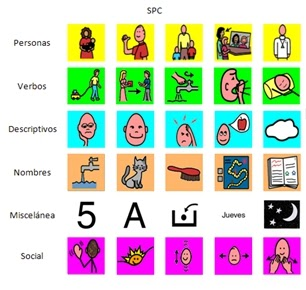
\includegraphics[width=0.7\linewidth]{Imagenes/Bitmap/SPCcolores}
	\caption{Ejemplo de categorías en SPC.}
	\label{fig:spccolores}
\end{figure}

\subsection{Blissymbolics}
Byssimbolics\footnote{\url{https://www.blissymbolics.org/index.php/about-blissymbolics}}
es un sistema de comunicación que fue usado por primera vez en 1971 para facilitar la comunicación con niños que padecían alguna discapacidad. Actualmente está compuesto por más de 5000 símbolos o  \textit{Bliss-Words} los cuales a su vez están compuestos por uno o más Caracteres-Bliss o  \textit{Bliss-Characters}. A pesar de que los 150 \textit{Bliss-Characters} que hay son sencillos de dibujar, requieren un periodo de aprendizaje para comprender su significado y así el de las \textit{Bliss-Words}. En la Figura \ref{fig:blisscharacters} vemos algunos \textit{Bliss-Characters} con su significado. \\
% TODO: \usepackage{graphicx} required

\begin{figure}[h!]
	\centering
	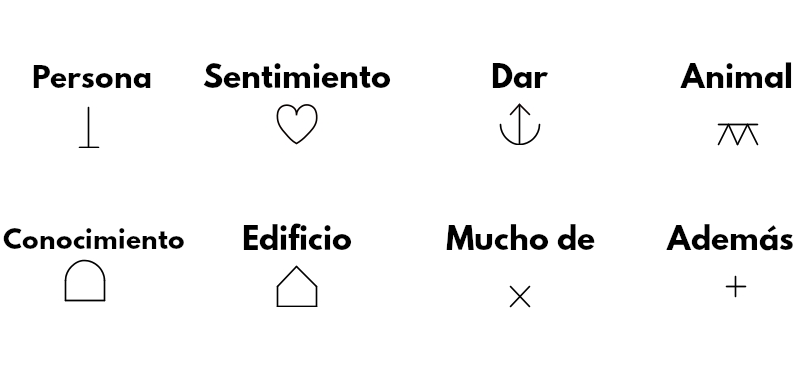
\includegraphics[width=0.8\linewidth]{Imagenes/Bitmap/BlissCharacters}
	\caption[Ejemplo de Bliss-Characters]{Ejemplo de Bliss-Characters.}
	\label{fig:blisscharacters}
\end{figure}
Una vez comprendido, en la Figura \ref{fig:blissword} vemos cómo se han combinado para generar \textit{Bliss-Words}. Destacar que el orden, el tamaño o la posición de los los Bliss-Characters, puede alterar su significado. Adicionalmente pueden estar agrupados de los mismos colores vistos en SPC.

% TODO: \usepackage{graphicx} required
\begin{figure}[h!]
	\centering
	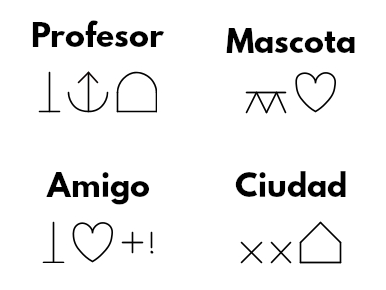
\includegraphics[width=0.4\linewidth]{Imagenes/Bitmap/BlissWord}
	\caption[Ejemplo de Bliss-Words]{Ejemplo de Bliss-Words.}
	\label{fig:blissword}
\end{figure}



\subsection{Sclera}
La principal característica de Sclera\footnote{\url{https://www.sclera.be/en/picto/overview}} frente a otros sistemas pictográficos es que sus pictogramas son menos coloridos pero cuentan con pictogramas más avanzados en cuanto a acciones representadas. Un ejemplo de ello se puede ver en la Figura \ref{fig:sclera} donde la acción de pedir atención se puede realizar de dos maneras posibles. Cuenta con un total de 11.497 pictogramas en español.

En la actualidad el desarrollo de Sclera está paralizado desde 2015.



% TODO: \usepackage{graphicx} required
\begin{figure}[h!]
	\centering
	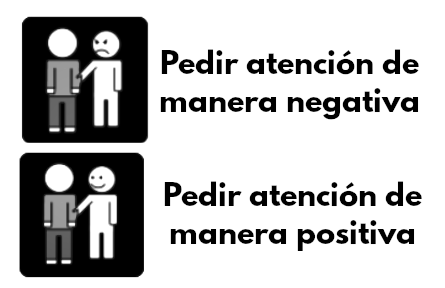
\includegraphics[scale=0.5]{Imagenes/Bitmap/Sclera}
	\caption{Ejemplo de acciones en Sclera.}
	\label{fig:sclera}
\end{figure}

\newpage
\subsection{Mulberry Symbols}
Mulbery Symbols\footnote{\url{https://mulberrysymbols.org/}} se creó con el propósito de ser un sistema pictográfico orientado a adultos ya que un gran porcentaje de dichos sistemas estaban pensados principalmente para niños y dificultaban la comunicación por falta de pictogramas. Como se observa en la Figura \ref{fig:mulberry} podemos ver ejemplos de pictogramas enfocados a adultos como cerveza o fumar.

Los pictogramas de Mulbery Symbols cuentan con 118 categorías incluyendo sustantivos, pronombres, verbos y con un total de 3.436 pictogramas.



% TODO: \usepackage{graphicx} required
\begin{figure}[h!]
	\centering
	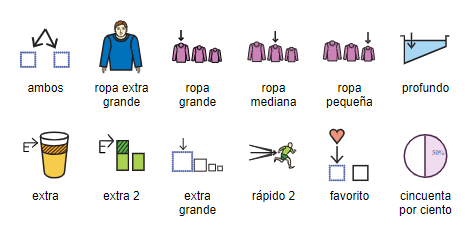
\includegraphics[scale=0.2]{Imagenes/Bitmap/Mulberry}
	\caption{Ejemplo de pictogramas de Mulberry.}
	\label{fig:mulberry}
\end{figure}

\newpage
\subsection{Minspeak}
Minspeak\footnote{\url{http://ares.cnice.mec.es/informes/18/contenidos/94.htm}}. es un sistema de comunicación alternativo creado por Bruce Baker en 1982. Difiere con los vistos anteriormente en que el significado de los iconos no viene preestablecido sino que es acordado entre usuario y logopeda. Es por ello que cada icono acordado tenga un significado distinto según la secuenciación de iconos. Por ejemplo en el caso de la Figura \ref{fig:minspeak} la asociación del icono casa junto a la cama, en ese orden podría ser interpretado como dormitorio. 

% TODO: \usepackage{graphicx} required
\begin{figure}[h!]
	\centering
	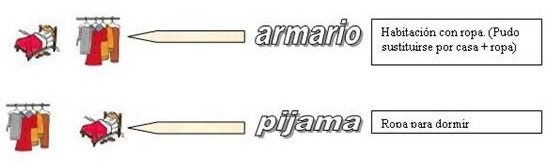
\includegraphics[width=0.7\linewidth]{Imagenes/Bitmap/Minspeak}
	\caption{Ejemplo de Minspeak.}
	\label{fig:minspeak}
\end{figure}

Como cada pictograma puede tener un significado distinto según su orden, se crearon Programas de Comunicación Minspeak (\textit{PAM}). Éstos se usan para cuando una casilla o icono haya sido seleccionada, se activen los posibles iconos con los que pueda tener algún tipo de relación. Inicialmente se creó hardware específico como aparece en la Figura \ref{fig:chatbox} con 16 celdas las cuales podía generar hasta 1024 mensajes, los teclados evolucionaron con más celdas y combinaciones, hasta pasar a teclados digitales implementados por software como PortaVoz\footnote{\url{http://www.terapia-ocupacional.com/articulos/Portavoz_JMLedesma.shtml}}.

% TODO: \usepackage{graphicx} required
\begin{figure}[h!]
	\centering
	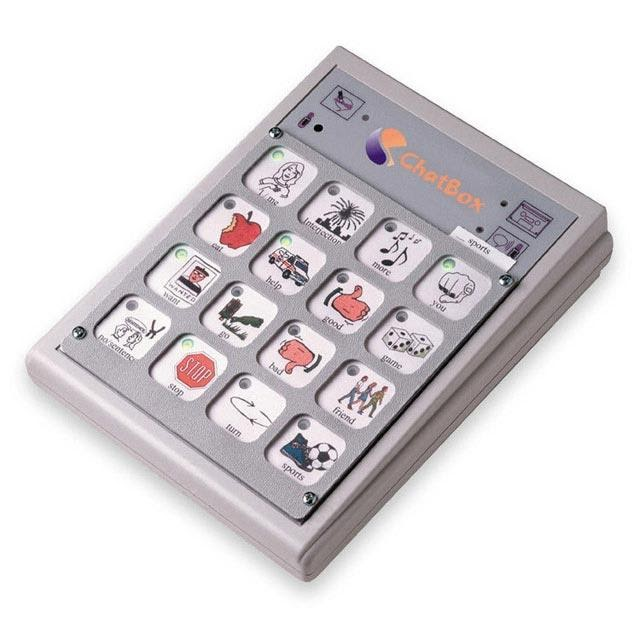
\includegraphics[width=0.4\linewidth]{Imagenes/Bitmap/ChatBox}
	\caption[ChatBox]{Panel de ChatBox}
	\label{fig:chatbox}
\end{figure}



\subsection{ARASAAC}

El portal Aragonés de Comunicación Aumentativa y Alternativa \\ (\textbf{ARASAAC})\footnote{\url{http://www.arasaac.org/}}
 surge en 2007 gracias a la colaboración entre el personal del CATEDU, el colegio público de educación Especial Alborada y del Centro Politécnico Superior de la Universidad de Zaragoza. Su objetivo era la creación de un sistema pictográfico de libre distribución que ayudara en el ámbito de la comunicación a todas aquellas personas que lo necesitasen.
Actualmente el portal de \textbf{ARASAAC} incluye fotografias, videos y cuenta con más de 39000 pictogramas tanto a color como en blanco y negro y con traducciones a 20 idiomas. También ofrece herramientas online con las que poder generar materiales como por ejemplo generador de calendarios, generador de tableros, creador de símbolos, etc.

A diferencia de otros sistemas pictográficos, \textbf{ARASAAC} permite una gran cantidad de opciones configurables como el color de fondo, marco o tiempo verbal, la Figura \ref{fig:configuarcion-arasaac} muestra todas las posibles opciones de configuración.



\begin{figure}[h!]
	\centering
	\includegraphics[width=0.7\linewidth]{Imagenes/Bitmap/Configuarción ARASAAC}
	\caption{Opciones de configuración de un pictograma.}
	\label{fig:configuarcion-arasaac}
\end{figure}



En la actualidad \textbf{ARASAAC} es uno de los sistemas pictográficos más utilizados a nivel de educación especial en España. Sus pictogramas se utilizan en colegios, universidades e incluso se han creado asociaciones para facilitar su implantación. CreaTea es una asociación en la Comunidad de Madrid cuyo objetivo es habilitar lugares como clínicas, restaurantes o ayuntamientos, para ayudar a la inclusión de personas con dificultades en la comunicación y concienciar a la sociedad.

También cabe destacar que \textbf{ARASAAC} ha recibido varios premios por su labor y que es una herramienta utilizada en varios países por lo que la cantidad de usuarios que colaboran es muy alta. Esto queda reflejado en la cantidad de pictogramas que se publican a la plataforma por parte de colaboradores sin ánimo de lucro y dichos pictogramas están constantemente actualizándose. Un ejemplo de ellos son los pictogramas que se han publicado debido a la pandemia como por ejemplo las Figuras \ref{fig:picto-mascarilla} y \ref{fig:picto-mascarilla-mal-colocada}.

\newpage
% TODO: \usepackage{graphicx} required
\begin{figure}[h!]
	\centering
	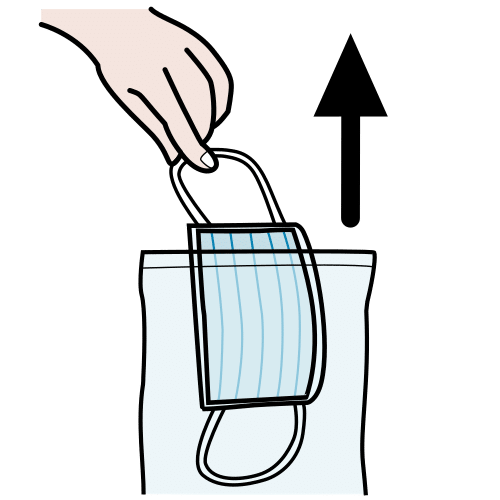
\includegraphics[width=0.2\linewidth]{Imagenes/Bitmap/Picto Mascarilla}
	\caption{Acción de sacar la mascarilla.}
	\label{fig:picto-mascarilla}
\end{figure}

\begin{figure}[h!]
	\centering
	
\includegraphics[width=0.2\linewidth]{Imagenes/Bitmap/Mascarilla mal colocada}
	\caption{Pictograma que representa mascarilla mal colocada.}
	\label{fig:picto-mascarilla-mal-colocada}
\end{figure}

En la Figura \ref{fig:arasaacpictos} podemos ver algunos ejemplos de pictogramas de \textbf{ARASAAC}, en situaciones o casos más cotidianos. Destacan la manera clara y concisa en la que están representados. 

% TODO: \usepackage{graphicx} required
\begin{figure}[h!]
	\centering
	
\includegraphics[width=0.7\linewidth]{Imagenes/Bitmap/ARASAACPictos}
	\caption{Ejemplo de pictogramas más típicos de ARASAAC.}
	\label{fig:arasaacpictos}
\end{figure}

La licencia de \textbf{ARASAAC} es de tipo \textit{Creative Commons (BY-NC-SA)} por lo que se podrá utilizar el material elaborado por ellos de cara a la implementación del Trabajo Fin de Grado. Utilizaremos sus pictogramas publicados en su página web y la API que han desarrollado para acceder a pictogramas de su base de datos.

\section{Editores de Tableros basados en Pictogramas}
\label{cap3:sec:editor-tableros}

A menudo estos tableros se realizan mediante piezas de papel recortadas y trabajar con ellas puede resultar engorroso, poco eficiente y apenas permiten modificaciones. Es por ello que la evolución lógica de los tableros pictográficos ha sido la digitalización. Para crear y editar tableros se han creado multitud de aplicaciones, a continuación estudiaremos sus características.

\subsection{Pictoselector}
Es una herramienta gratuita para crear agendas visuales. Recopila más de 28.000 provenientes de \textbf{Sclera}, \textbf{Mulberry}, \textbf{ARASAAC}, etc. Al crear un proyecto, permite cargar una plantilla o crear una desde cero. Se puede modificar el número de filas y columnas, la posición del texto y el tamaño del borde de los pictogramas.
\footnote{\url{ https://www.pictoselector.eu/es/ }}

% TODO: \usepackage{graphicx} required
\begin{figure}[h!]
	\centering
	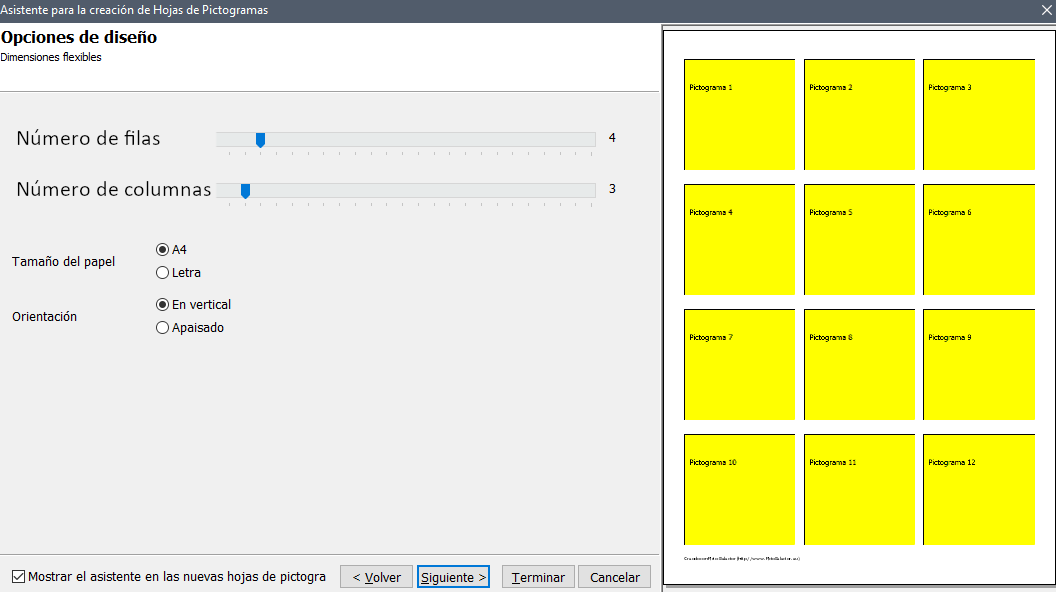
\includegraphics[width=0.7\linewidth]{Imagenes/Bitmap/Pictoselector Tablero}
	\caption{Ventana donde se edita el tamaño de la cuadrícula.}
	\label{fig:pictoselector-tablero}
\end{figure}


Una vez creado el tablero, podemos insertar en su cuadrícula distintos elementos, muchos de ellos en forma de pictograma. Para facilitar esta tarea, la cabecera de la aplicación contiene acceso directo a la inserción de pictogramas



Como podemos ver, de izquierda a derecha, existe un buscador de pictogramas que incluye la función de filtrar por juego de pictogramas. Además de poder editar ligeramente el picto ya sea coloreándolo o añadiendo un signo de pasado, presente o plural. Para el marcaje de tiempo pueden incluirse con facilidad pictogramas de reloj que marcan la hora y de duración que marcan un intervalo de tiempo. Adicionalmente se puede importar imágenes propias, códigos QR , texto o emoticonos.

% TODO: \usepackage{graphicx} required
\begin{figure}[h!]
	\centering
	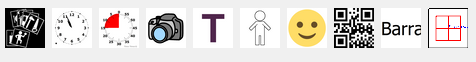
\includegraphics[width=0.7\linewidth]{Imagenes/Bitmap/Ribbon Pictoselector}
	\caption{Barra de inserción de pictogramas.}
	\label{fig:ribbon-pictoselector}
\end{figure}

% TODO: \usepackage{graphicx} required
\begin{figure}[h!]
	\centering
	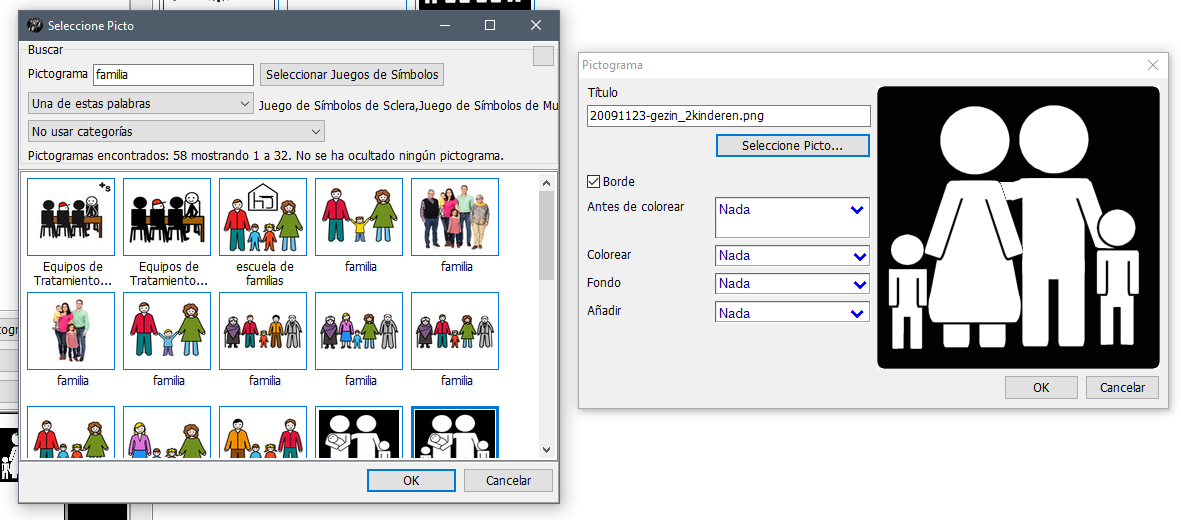
\includegraphics[width=0.7\linewidth]{Imagenes/Bitmap/Editor y buscador de pictoselector}
	\caption{Buscador y editor de Pictogramas.}
	\label{fig:editor-y-buscador-de-pictoselector}
\end{figure}




El mayor inconveniente de la aplicación, pese a ser muy completa respecto a la búsqueda y edición de pictos, es su limitación de colocación a una cuadrícula.

\subsection{Editor ARASAAC}
La página web de ARASAAC cuenta con herramientas online las cuales podemos usar para generar materiales .
\begin{itemize}
\item \textbf{Creador de animaciones}: genera una animación con los pictogramas que queramos en formato GIF o SWF. También permite configurar el intervalo entre los pictogramas y el número de repeticiones que hará.

\item \textbf{Creador de símbolos}: permite la personalización de pictogramas donde podremos cambiar el nombre del pictograma, poner su traducción, modificar la fuente del texto, poner un marco, ampliar la imagen y cambiar el fondo.

\item \textbf{Generador de frases}: consta de un total de tres pasos a seguir, el primero de ellos consiste en seleccionar las palabras que queramos traducir a pictogramas, el segundo paso nos mostrará todos los pictogramas asociados para cada palabra introducida y deberemos seleccionar el que más nos guste y el tercer paso aparecerán todos los pictogramas colocados en una tabla la cual podremos modificar.
\footnote{\url{ http://www.arasaac.org/herramientas.php }}

% TODO: \usepackage{graphicx} required
\begin{figure}[h!]
	\centering
	
\includegraphics[width=0.7\linewidth]{Imagenes/Bitmap/Frase ARASAAC}
	\caption{Ejemplo con generador de frases.}
	\label{fig:frase-arasaac}
\end{figure}


\item \textbf{Generador de horarios}: genera un horario donde previamente tendremos que configurar una plantilla con los días, horas, el formato (horizontal o vertical), idioma, bordes del horario, texto para cada día y hora y la opción de insertar un pictograma en función de su día y hora.

\item \textbf{Generador de calendarios}: genera un calendario donde tendremos que especificar el mes, año e idioma deseado. Al igual que en el generador de horarios permite la opción de modificar el texto, colores, bordes y la posibilidad de poner un pictograma para cada día del mes.

\item \textbf{Generador de tableros}: crea un tablero con el número de filas y columnas deseado donde para cada casilla podremos insertar un pictograma. Al igual que en otras herramientas permite la modificación de colores, bordes y  texto del tablero.

\item \textbf{Creador de juegos}: genera una plantilla en formato .rtf para poder jugar al bingo, oca, dominós y dominós encadenados con los pictogramas que deseemos.
\end{itemize}

% TODO: \usepackage{graphicx} required
\begin{figure}[h!]
	\centering
	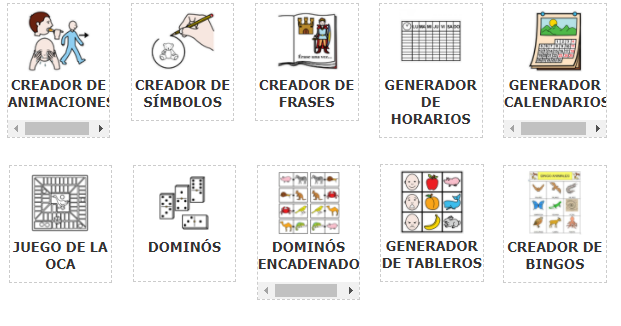
\includegraphics[width=0.4\linewidth]{Imagenes/Bitmap/Tableros ARASAAC}
	\caption[Tableros web ARASAAC]{Herramientas online que ofrece ARASAAC.}
	\label{fig:tableros-arasaac}
\end{figure}

\newpage
\subsection{Piktoplus}
Se trata de una aplicación para dispositivos Android. Su particularidad es que permite la creación de un avatar tridimensional personalizable\footnote{\url{http://www.aulautista.com/2013/12/05/piktoplus-un-comunicador-android-muy-especial/ }}. Dicho avatar será usado en los tableros pictográficos pues será quien protagonice las acciones. Permite registrar múltiples usuarios, cada uno con su propio avatar. Otra particularidad de Piktoplus son los sub-tableros. \footnote{\url{https://fatimamikel.wordpress.com/2014/04/17/piktoplus-2/ }}  Por ejemplo, en la Figura \ref{fig:piktoplus1}  hay un tablero con dos pictogramas, “Estoy” y “Me duele”.


% TODO: \usepackage{graphicx} required
\begin{figure}[h!]
	\centering
	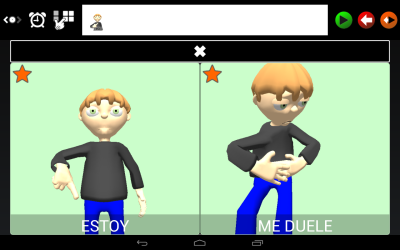
\includegraphics[width=0.5\linewidth]{Imagenes/Bitmap/Piktoplus1}
	\caption[Pictoplus tablero]{Ejemplo de tablero en Piktoplus}
	\label{fig:piktoplus1}
\end{figure}

En el caso que pusemos sobre estoy, se desplegará un sub-tablero dentro del mismo tablero con cuatro pictogramas como se representa en la Figura \ref{fig:piktoplus2}.


% TODO: \usepackage{graphicx} required
\begin{figure}[h!]
	\centering
	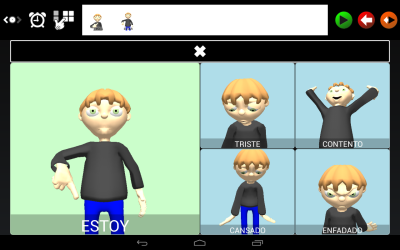
\includegraphics[width=0.5\linewidth]{Imagenes/Bitmap/Piktoplus2}
	\caption[Subtablero Piktoplus]{Subtablero en Piktoplus}
	\label{fig:piktoplus2}
\end{figure}


Respecto a la creación y edición de tableros, se trata de una cuadrícula sobre la cual se colocan los pictogramas, además permite aumentar el tamaño de los pictos. Por ejemplo “Estoy” ocupa cuatro celdas más que “Contento”. 

Actualmente esta aplicación no está disponible para descargar en tiendas de aplicaciones  habituales y su desarrollo ha cesado desde 2018. Aunque no esté disponible, plantea una idea muy interesante como la posibilidad de desplegar un sub-tablero a partir de un pictograma para mostrar pictogramas relacionados entre ellos.


\subsection{Pictar}
La aplicación Pictar permite generar una secuencia de pictogramas traduciendo una frase introducida por el usuario. Esa secuencia de pictogramas se podrán colocar automáticamente en el tablero.


El tablero está compuesto por casillas, separadas en filas y columnas permitiendo añadir más elementos.

En el tablero tendremos únicamente la opción de eliminar la casilla o borrar su contenido.En el lateral izquierdo se encuentra un buscador de pictogramas de la base de datos de ARASAAC. Los cuales se pueden colocar en el tablero ya sea sustituyendo pictogramas existentes o rellenando casillas vacías.
\footnote{\url{ http://hypatia.fdi.ucm.es/pictar/ }}

% TODO: \usepackage{graphicx} required
\begin{figure}[h!]
	\centering
	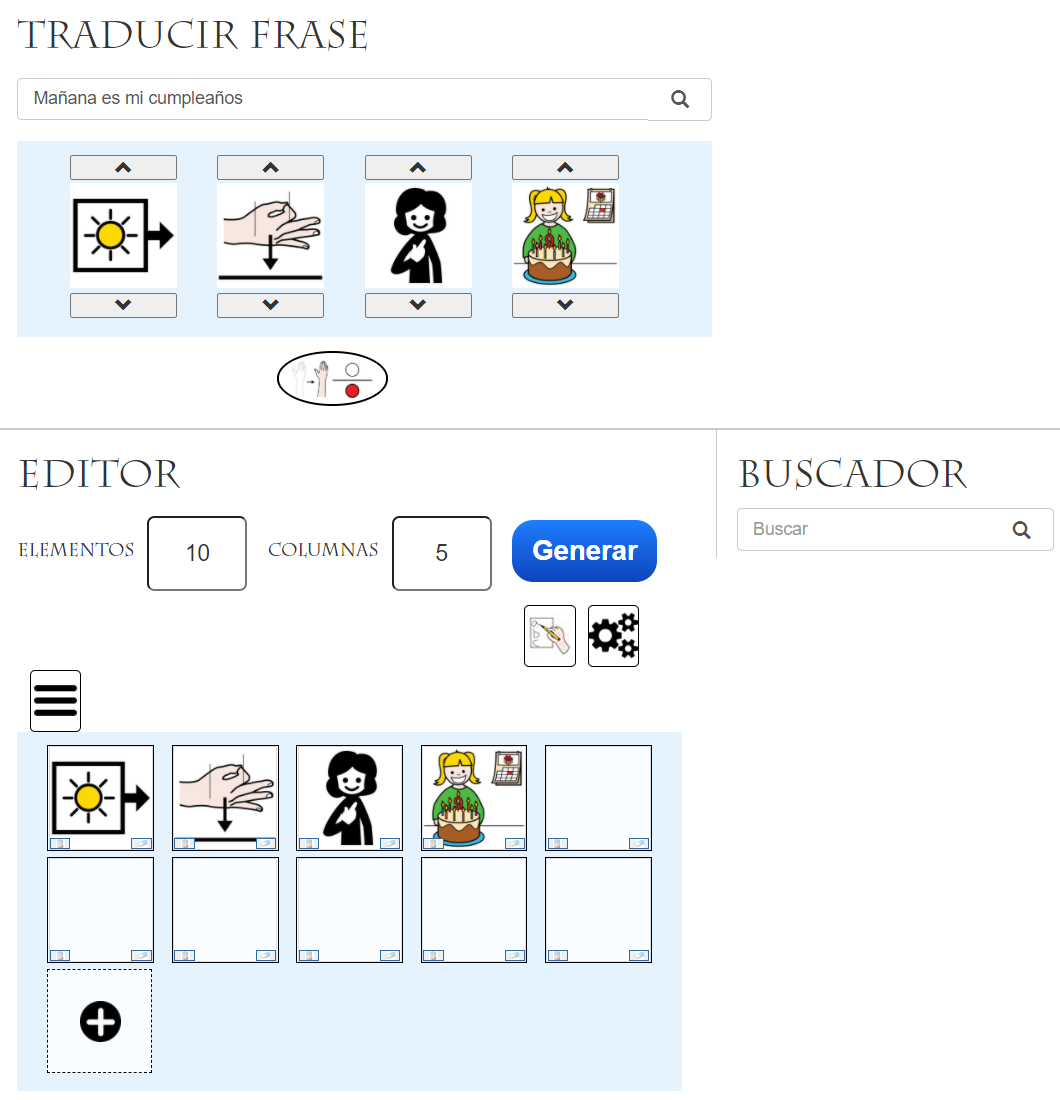
\includegraphics[width=0.7\linewidth]{Imagenes/Bitmap/Pictar}
	\caption{Menú de la aplicación Pictar.}
	\label{fig:pictar}
\end{figure}

\newpage
\subsection{Pictableros}
\footnote{\url{ https://holstein.fdi.ucm.es/picto-tableros/  }}
Pictableros es una aplicación web de edición y creación de tableros y plantillas para pictogramas. Tiene dos partes diferenciadas:

\begin{itemize}
	\item Las plantillas sirven para que otros usuarios que quieran crear un tablero similar puedan sustituir con facilidad los pictogramas. Por ejemplo en la Figura \ref{fig:pictableros1} existe una plantilla de tablero para elegir un deporte, dicha plantilla puede ser modificada para sustituir el pictograma de balonmano por tenis. Estas plantillas pueden ser públicas o privadas.
	
	\item Los tableros públicos no pueden ser modificados, aunque  se puede crear una copia de ellos y modificarse para superponer símbolos (Bien, mal, amarillo, azul)
	

\end{itemize}

	% TODO: \usepackage{graphicx} required
	\begin{figure}[h!]
		\centering
		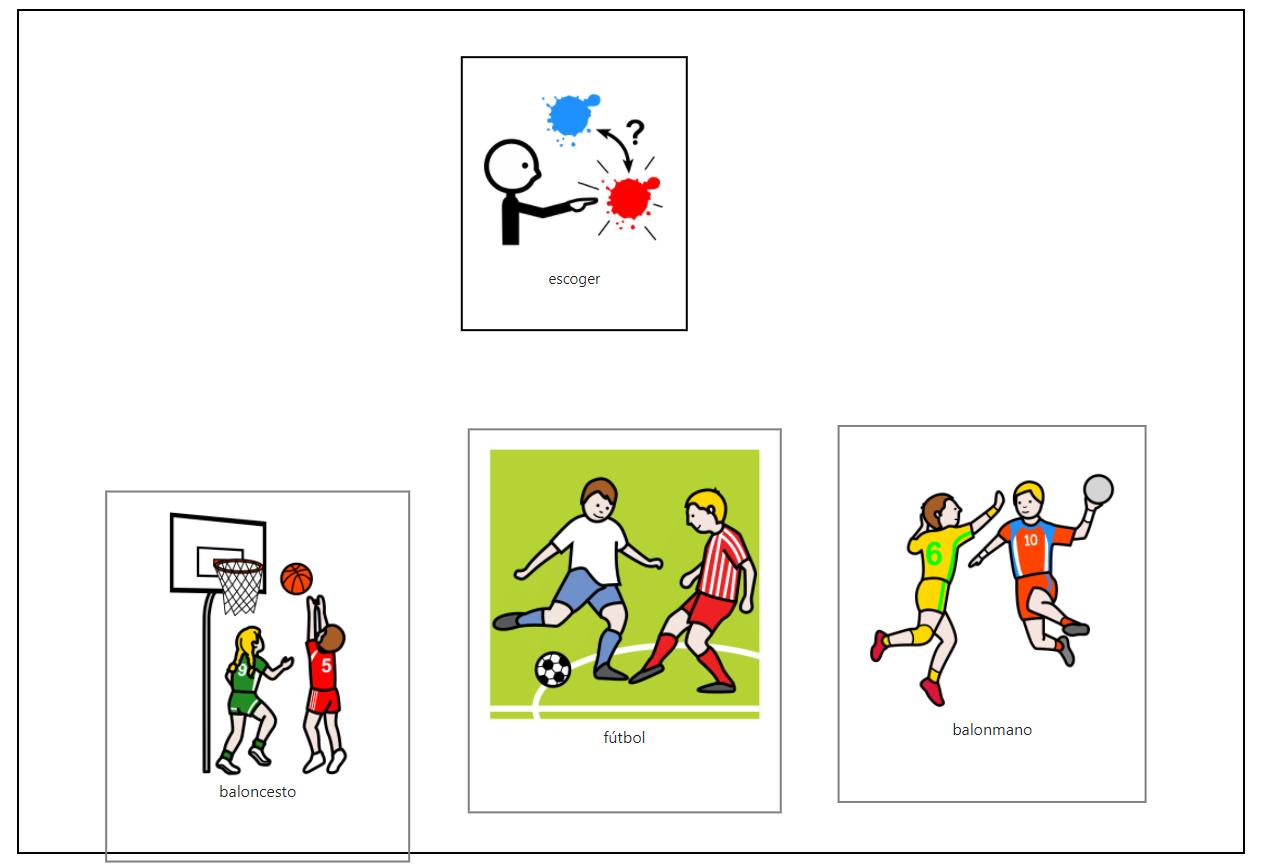
\includegraphics[width=0.7\linewidth]{Imagenes/Bitmap/pictableros1}
		\caption{Plantilla de elección de deporte.}
		\label{fig:pictableros1}
	\end{figure}
	
	
	% TODO: \usepackage{graphicx} required
	\begin{figure}[h!]
		\centering
		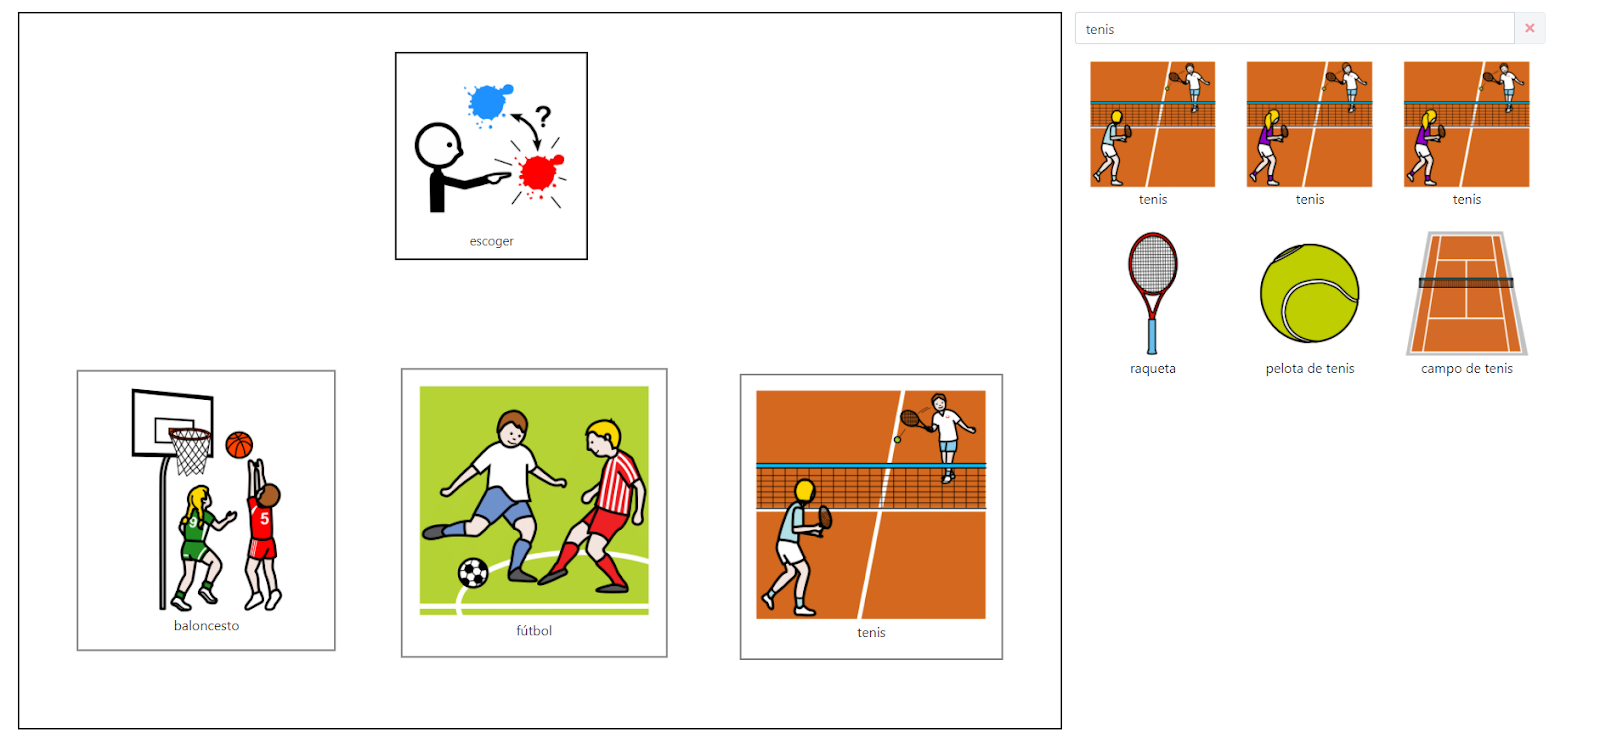
\includegraphics[width=0.7\linewidth]{Imagenes/Bitmap/pictableros2}
		\caption[Edición de plantilla en Pictableros]{Edición de plantilla de selección de deporte, sustituimos balonmano por tenis, haciendo uso del buscador de pictogrmas.}
		\label{fig:pictableros2}
	\end{figure}
	
	% TODO: \usepackage{graphicx} required
	\begin{figure}[h!]
		\centering
		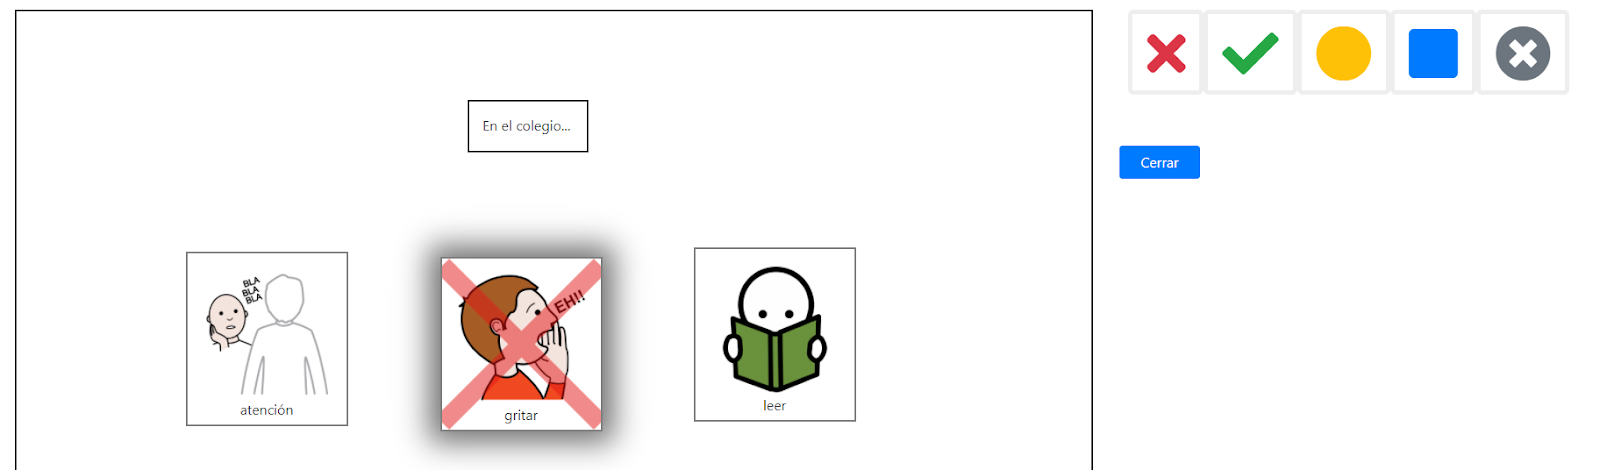
\includegraphics[width=0.7\linewidth]{Imagenes/Bitmap/pictableros3}
		\caption[Edición plantilla en Pictableros]{Edición de tableros, permite superponer un signo al pictograma.}
		\label{fig:pictableros3}
	\end{figure}
	

	


\newpage	
\subsection{Symbo Talk}

SymboTalk permite la creación de tableros de comunicación aumentativa y locución de tableros y pictogramas mediante su aplicación web o dispositivos móviles como Android e iOS.
\footnote{\url{  https://civat.es/app/symbo-talk/ }}
\footnote{\url{   http://aulaabierta.arasaac.org/symbotalk-0-inicio-2  }}
SymboTalk ofrece dos modos de usuario:

\begin{itemize}
	\item \textbf{Modo edición}: permite la creación de pictogramas, construir tableros, buscar pictogramas en un buscador. También ofrece la opción de crear un perfil y poder guardar todos los tableros que hayamos realizado.
	
	\item \textbf{Modo usuario}: pensado para que el usuario pueda comunicarse de una forma más fácil e intuitiva.
	
\end{itemize}

% TODO: \usepackage{graphicx} required
\begin{figure}[h!]
	\centering
	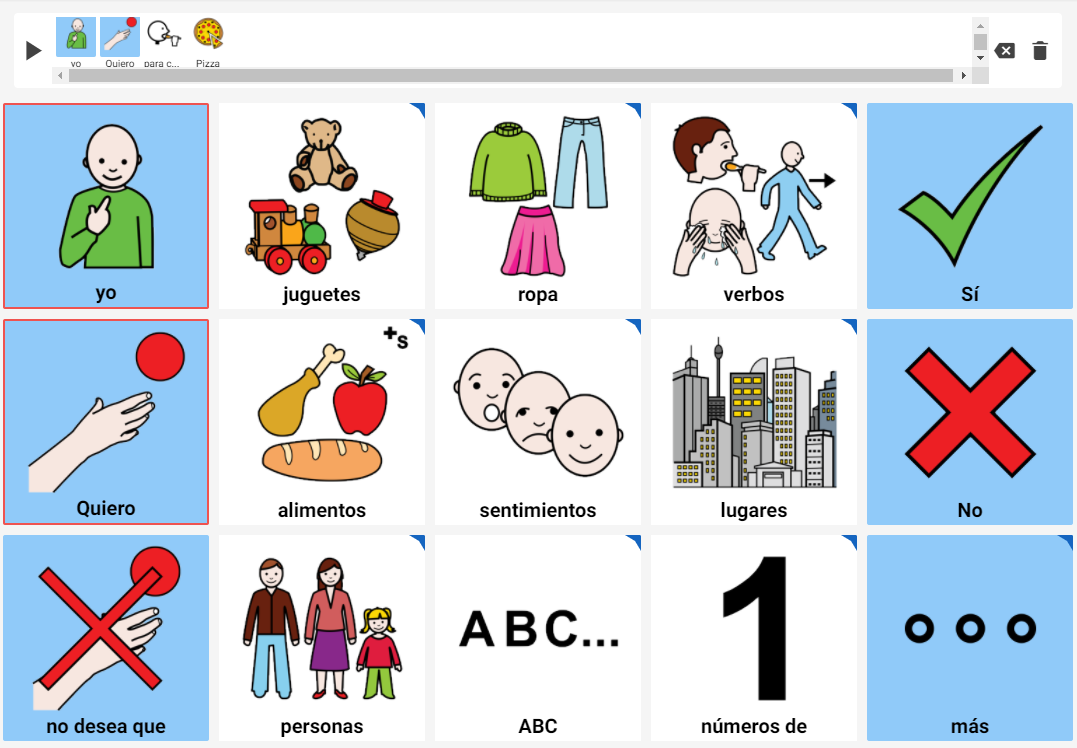
\includegraphics[width=0.7\linewidth]{Imagenes/Bitmap/SymboTalk}
	\caption{Pantalla principal de la aplicación Symbo Talk.}
	\label{fig:symbotalk}
\end{figure}

\newpage
\subsection{LetMe Talk}

LetMe Talk es una aplicación para dispositivos Android e iOS que permite generar frases a partir de pictogramas seleccionados. Tiene un total de 9.000 pictogramas de \textit{ARASAAC} y ofrece la posibilidad de añadir imágenes con un texto descriptivo con la cámara del dispositivo.

\footnote{\url{ https://www.letmetalk.info/es}}
% TODO: \usepackage{graphicx} required
\begin{figure}[h!]
	\centering
	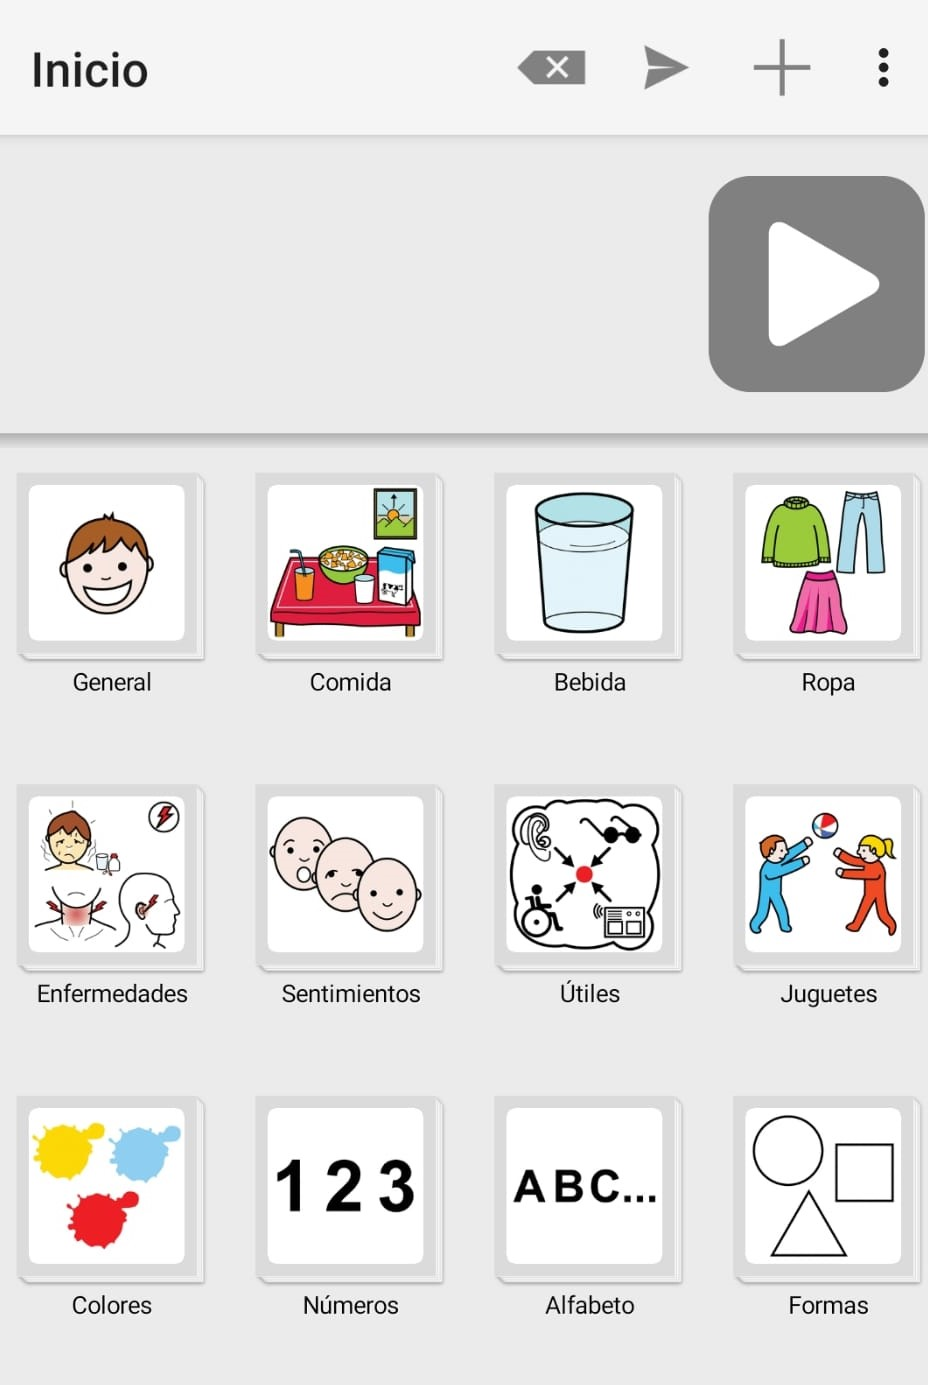
\includegraphics[width=0.7\linewidth]{Imagenes/Bitmap/LetMeTalk}
	\caption{Menú de la aplicación en Android de LetMe Talk.}
	\label{fig:letmetalk}
\end{figure}

\newpage

\section*{Análisis de los resultados}



\begin{table}[]
	\centering
	\resizebox{14cm}{!} {
		\begin{tabular}{|l|l|l|l|l|l|l|}
			\hline
			
			\textbf{Programas} & \textbf{Disponible} & \textbf{Actualizado} & \textbf{Dispositivos} & \textbf{{\begin{tabular}[c]{@{}l@{}}\\ Permite editar \\ pictogramas \\ \\\end{tabular}}}  & \textbf{Precio} & \textbf{Idiomas} \\  \hline
			
			\textbf{Pictoselector} &Sí  &Sí  &PC y MAC  &Sí &Gratuito &{\begin{tabular}[c]{@{}l@{}}\\ES, EN, DU, FR, \\ PT, IT\\ \\\end{tabular}} \\ \hline
			\textbf{Editor ARASAAC} &Sí  &Sí  &{\begin{tabular}[c]{@{}l@{}}\\PC, MAC, Android, \\ iOS y Web \end{tabular}}  &Sí &Gratuito &{\begin{tabular}[c]{@{}l@{}}\\ES, EN, DU, FR, \\ PT, BZ, IT, RO, \\ PL, CN, AR, RU, \\ BG, CRO, NLD\\ \\\end{tabular}} \\ \hline
			\textbf{Piktoplus} &No  &No  &Android  &No &139€ &{\begin{tabular}[c]{@{}l@{}} \\ES \\ \\ \end{tabular}}\\ \hline
			\textbf{BoardMaker} &Sí  &Sí  &PC y MAC  &No &300€ &{\begin{tabular}[c]{@{}l@{}} \\ES, EN, PT \\ \\\end{tabular}}\\ \hline
			\textbf{Pictar} &Sí  &{\begin{tabular}[c]{@{}l@{}}\\La web no, \\los pictogramas sí\end{tabular}}  &Web  &No &Gratuito &{\begin{tabular}[c]{@{}l@{}} \\ES \\ \\ \end{tabular}}\\ \hline
			\textbf{Pictableros} &Sí  &{\begin{tabular}[c]{@{}l@{}}\\La web no, \\los pictogramas sí\end{tabular}}   &Web  &Sí &Gratuito &{\begin{tabular}[c]{@{}l@{}} \\ES \\ \\ \end{tabular}}\\ \hline
			\textbf{SymboTalk} &Sí  &No  &Web, Android e iOS  &No &Gratuito &{\begin{tabular}[c]{@{}l@{}} \\ES, EN, HEBR \\ \\ \end{tabular}}\\ \hline
			\textbf{LetMeTalk} &Sí  &No  &Android e iOS  &No &Gratuito &{\begin{tabular}[c]{@{}l@{}} \\ES, AR, DE, EN, \\ IT, FR, PL, PT, \\ RU, RO, SW, CN \\ \\\end{tabular}} \\ \hline
			
		\end{tabular}
	}
\caption{\label{tab:table-name}Tabla comparativa entre los distintos editores de tableros basados en pictogramas}
\end{table}


Puestos todas las herramientas en comparación, podemos extraer algunos resultados. Actualmente la mayoría de estas herramientas están disponibles y con una base de datos de pictogramas actualizada. Los más completos o que ofrecen más opciones, están disponibles para ordenadores aunque en dispositivos móviles hay mayor oferta  de aplicaciones, generalmente ofrecen pocas opciones. Además de las aplicaciones de dispositivos, las más actualizadas son las que se pueden acceder en formato web.

Aunque a pesar de todo, el factor determinante es el precio. Las aplicaciones que no son gratuitas suelen tener un precio desorbitado o que muchas familias o docentes no pueden permitirse, por ello que una aplicación sea gratuita es determinante. Respecto a los idiomas, destacan el español y el inglés como idiomas predominantes entre las aplicaciones. 

Como conclusión, creemos que la herramienta que desarrollemos debería cumplir las siguientes características. Debe ser gratuita, disponible desde navegador web, con edición de pictogramas, una base de datos de éstos actualizada y que esté disponible como mínimo en español e inglés. 